\documentclass[tikz,xcolor=table,aspectratio=1610]{beamer}
\usepackage[english]{babel}
\makeatletter
\makeatother
\usetheme[progressbar=frametitle,subsectionpage=progressbar,block=fill]{metropolis}
\RequirePackage{MyTalkSty}
%\input{Diagrams}
\setbeameroption{show notes} % Speaker notes
%\setbeameroption{show only notes}     %  only notes
% \setbeameroption{hide notes}         %  

\thispagestyle{empty}

%###########################################
%############ Background (global) ##########
%###########################################
\setbeamertemplate{background canvas}{
    \transparent{0.8}
    \begin{picture}(0,275.0)
        \hspace{9.2cm}
        \begin{minipage}[b]{1.0\textwidth}
           % \href{https://}{\includegraphics[scale=0.07]{../Figures/Logos/.png}}
           % \href{https://www.}{\includegraphics[scale=0.05]{../Figures/Logos/.png}}
           % \hspace{7.5cm}
           % \href{https://}{\includegraphics[width=0.15\linewidth]{../Figures/Logos/.png}}
        \end{minipage}
    \end{picture}
}

%###########################################
%################# Title data ##############
%###########################################
\newcommand{\tit}{Title}
\newcommand{\event}{Event Name}
\newcommand{\name}{Author} % \orcidlinkicon{number}
\newcommand{\instshort}{Institute}
\newcommand{\inst}{\href{https://www.}{\instshort}}
\newcommand{\colabList}{et al.}
\newcommand{\logoi}{\href{https://www.}{includegraphics path 1}} %\includegraphics[scale=0.13]{../Figures/Logos/.....png}
\newcommand{\logoii}{\href{https://www.}{includegraphics path 2}}
\newcommand{\logoiii}{\href{https://www.}{includegraphics path 3}}

%###########################################
%################### Title #################
%###########################################
\thispagestyle{empty}
\title[\tit]{\huge \textcolor{cobalt}{\tit} }
\subtitle{\event}
\author[\name]{\name}
\institute[\instshort]{%
  \affiliationInline
    {{\bf\color{cobalt!70!black} In collaboration with: \colabList}}
    {\arxiv{\href{https://arxiv.org/abs/XXXX.YYYYY}{arXiv:XXXX.YYYYY}}}
    {\transparent{0.8}\hspace{-0.5cm}\logoi\logoii\logoiii}%
    {}%
}
\date{ add Date}

%###########################################
%############## Document start #############
%###########################################
\begin{document}

%###########################################
%###########################################
%###########################################
\begin{frame}
\maketitle
\end{frame}

%###########################################
%###########################################
%###########################################
\setcounter{framenumber}{0}

%###########################################
%###########################################
%###########################################
\setbeamertemplate{background canvas}{ \transparent{0.0}\hspace{8.5cm}
\begin{picture}(0,247)
\end{picture}
}

%###########################################
%############## Overview / TOC #############
%###########################################
\begin{frame}\frametitle{Contents}
\scriptsize
\tableofcontents%[currentsection] %, hideothersubsections]
\end{frame}

%###########################################
%###########################################
%###########################################
\setbeamertemplate{background canvas}{
    \transparent{0.8}
    \begin{picture}(0,250.0)
        \hspace{2.2cm}
        \begin{minipage}[b]{1.0\textwidth}
            Add an important text
        \end{minipage}
    \end{picture}
}

%###########################################
%################### Section ###############
%###########################################
\section{section}

%###########################################
%############ Section landing ##############
%###########################################
\setbeamertemplate{background canvas}{
    \transparent{0.8}
    \begin{picture}(0,250.0)
        \hspace{9.2cm}
        \begin{minipage}[b]{1.0\textwidth}
        \end{minipage}
    \end{picture}
}

%###########################################
%############## Fixed TikZ #################
%###########################################
\begin{frame}{My fixed TikZ frame}
\FixedTikZLayout
  {% #1 image1
   %\includegraphics[scale=1.0]{path/to/img1}
  }
  {Box 1 text}
  {Box 2 text}
  {Box 3 text}
  {% #5 image2
   %\includegraphics[scale=0.068]{path/to/img2}
  }
  {Right-side explanation text.}
\end{frame}
\note{\scriptsize Here: speaker's notes}
%###########################################
%###########################################
%###########################################
\begin{frame}{Variant layout}
\FixedTikZLayoutParam{Image 1}{Box 1}{Box 2}{Box 3}{Image 2}{Explanation Text}
\end{frame}

%###########################################
%############## Layout basics ##############
%###########################################
\begin{frame}{Three-column example}
\footnotesize\justifying
\ThreeCol{0.33}{0.34}{0.33}{
\textbf{Column 1}
\begin{firstitemize}
  \item Item A
  \item Item B
\end{firstitemize}
}{
\textbf{Column 2}
\begin{remark}[Note]
A remark box can live inside a column.
\end{remark}
}{
\textbf{Column 3}
}
\end{frame}

%###########################################
%############## Math primitives ############
%###########################################
\begin{frame}{Boxed equations: reusable primitives}
\footnotesize\justifying

\[
\mBox[cyan!10]{a^2+b^2}
=
\mBox[blue!10]{c^2}
\qquad
\text{and}\qquad
\mBox[red!5]{A}
\le
\mBox[green!10]{B}
\]

\medskip
\begin{myNote}[Tip]
Use \texttt{\textbackslash mBox[<color>]\{<math>\}} inside equations to highlight objects consistently.
\end{myNote}

\end{frame}

%###########################################
%###########################################
%###########################################
\begin{frame}{Using CalloutTo}
\footnotesize\justifying

\[
\mathcal{D}
=
\frac{%
  \mBoxN[cyan!10]{Abox}{A}\,
  \mBoxN[red!5]{Bbox}{\mathcal{B}}%
}{%
  \mBoxN[blue!10]{Cbox}{C}%
}
\]
\begin{tikzpicture}[remember picture,overlay]
  \CalloutTo{callA}{($(Abox.north west)+(-0.6cm,0.7cm)$)}
    {\textbf{\footnotesize A}}{cyan!10}{Abox.west}{out=200,in=-20}

  \CalloutTo{callB}{($(Bbox.north east)+(0.6cm,0.7cm)$)}
    {\textbf{\footnotesize B}}{red!5}{Bbox.east}{out=-20,in=200}

  \CalloutTo{callC}{($(Cbox.south)+(-1.0cm,-0.5cm)$)}
  {\textbf{\footnotesize C}}{blue!10}{Cbox.south}{out=-45,in=-45}
\end{tikzpicture}
\end{frame}

%###########################################
%###########################################
%###########################################
\subsection{subsection}

%###########################################
%############ Subsection landing ###########
%###########################################
\setbeamertemplate{background canvas}{
\transparent{0.8}
\begin{picture}(0,200.0)
\hspace{8.7cm}
\begin{minipage}[b]{0.5\textwidth}
% iluikyujdfgafgwr
\end{minipage}
\end{picture}
}

%###########################################
%############ Watermark examples ###########
%###########################################
\begin{frame}{Preliminary Mark}
\Watermark[Preliminary]{0.10}{5}{35}{-3cm}{0cm} %or \PreliminaryMark

\begin{columns}
  \begin{column}{0.5\textwidth}
    % contenido
  \end{column}
  \begin{column}{0.5\textwidth}
    \justifying
    % contenido
  \end{column}
\end{columns}
\end{frame}

%###########################################
%###########################################
%###########################################
\begin{frame}{}
  \begin{innerblockplain}
    %
  \end{innerblockplain}
\end{frame}

%###########################################
%###########################################
%###########################################
\begin{frame}{Three columns + Preliminary}
\Watermark[Preliminary]{0.10}{5}{35}{-0cm}{0cm}

\footnotesize\justifying
\ThreeCol{0.30}{0.40}{0.30}{
\textbf{Inputs}
\begin{firstitemize}
  \item Data
  \item Simulation
\end{firstitemize}
}{
\textbf{Method}
\begin{firstitemize}
  \item Selection
  \item Fits
  \item Systematics
\end{firstitemize}
}{
\textbf{Outputs}
\begin{firstitemize}
  \item Limits
  \item Plots
\end{firstitemize}
}
\end{frame}

%###########################################
%############ Separator utilities ##########
%###########################################
\begin{frame}{Three-column example}
\footnotesize\justifying
\ThreeColSep{
  % col1
}{
  % col2
}{
  % col3
}
\end{frame}

%###########################################
%###########################################
%###########################################
\begin{frame}{Two columns + separator}
\footnotesize\justifying
\begin{columns}[T,onlytextwidth]
  \begin{column}{0.61\textwidth}
    Left content
  \end{column}

  \ColSep{0.5pt}

  \begin{column}{0.37\textwidth}
    Right content
  \end{column}
\end{columns}
\end{frame}

%###########################################
%###########################################
%###########################################
\begin{frame}{Two columns + separator}
\footnotesize\justifying
\begin{columns}[T,onlytextwidth]
  \begin{column}{0.61\textwidth} ... \end{column}
  \ColSepTikZ{0.6pt}
  \begin{column}{0.37\textwidth} ... \end{column}
\end{columns}
\end{frame}

%###########################################
%###########################################
%###########################################
\begin{frame}{Three columns + separators}
\footnotesize\justifying
\begin{columns}[T,onlytextwidth]
  \begin{column}{0.31\textwidth} Col 1 \end{column}
  \ColSep{0.4pt}
  \begin{column}{0.33\textwidth} Col 2 \end{column}
  \ColSep{0.4pt}
  \begin{column}{0.31\textwidth} Col 3 \end{column}
\end{columns}
\end{frame}

%###########################################
%############ Lists / boxes demos ##########
%###########################################
\begin{frame}{Lists}
\footnotesize\justifying

\begin{firstitemize}
  \item First level (\texttt{firstitemize})
  \begin{seconditemize}
    \item Second level (\texttt{seconditemize})
    \begin{thirditemize}
      \item Third level (\texttt{thirditemize})
      \begin{myitemize}
        \item Bullet style (\texttt{myitemize})
      \end{myitemize}
    \end{thirditemize}
  \end{seconditemize}
  \item Another first-level item
\end{firstitemize}

\end{frame}

%###########################################
%###########################################
%###########################################
\begin{frame}{Remark box}
\footnotesize\justifying

\begin{remark}[Work in progress]
This box is a \texttt{tcolorbox} environment called \texttt{remark}. Use it for warnings or short messages.
\end{remark}

\medskip

\begin{firstitemize}
  \item Put regular text outside the box as usual.
\end{firstitemize}

\end{frame}

%###########################################
%############ Different BG example #########
%###########################################
\setbeamertemplate{background canvas}{
    \transparent{0.8}
    \begin{picture}(0,270.0)
        \hspace{0.8cm}
        \begin{minipage}[b]{1.0\textwidth}
        \end{minipage}
    \end{picture}
}

%###########################################
%###########################################
%###########################################
\begin{frame}{Definition}
\footnotesize\justifying

\begin{defn}[Name]
A \emph{definition} box is for key concepts you will reference later.
\end{defn}

\end{frame}

%###########################################
%###########################################
%###########################################
\begin{frame}{Note box}
\footnotesize\justifying

\begin{columns}
\begin{column}{0.62\textwidth}
\begin{firstitemize}
  \item Main content on the left.
  \item Use \texttt{myNote} on the right for a compact takeaway.
\end{firstitemize}
\end{column}

\begin{column}{0.38\textwidth}
\begin{myNote}[Take-home]
A short takeaway, constraint, or reminder that should stand out.
\end{myNote}
\end{column}
\end{columns}

\end{frame}

%###########################################
%###########################################
%###########################################
\begin{frame}{Two-column layout example}
\footnotesize\justifying

\begin{columns}
\begin{column}{0.62\textwidth}
\textbf{Key points}
\begin{firstitemize}
  \item Point 1
  \item Point 2
\end{firstitemize}
\end{column}

\begin{column}{0.38\textwidth}
\begin{remark}[Caveat]
State an important limitation or assumption here.
\end{remark}
\end{column}
\end{columns}

\end{frame}

%###########################################
%############### Tables demo ###############
%###########################################
\begin{frame}{General table: multi-column + multi-row}
\footnotesize

\begin{center}
\setlength{\tabcolsep}{7pt}
\renewcommand{\arraystretch}{1.25}

{\mdseries

\colorlet{RowVal}{cobalt!25}      % blue-ish rows with values
\colorlet{RowNote}{gray!25}      % gray rows with notes
\colorlet{RowHead}{gray!85}      % header bar
\colorlet{RowComment}{cobalt!45}  % emphasized full-row comment

\begin{tabular}{l c c c c c}
\toprule

\multicolumn{1}{c}{\textbf{Category}} &
\multicolumn{3}{c}{\textbf{Group A}} &
\multicolumn{2}{c}{\textbf{Group B}} \\
\cmidrule(lr){2-4}\cmidrule(lr){5-6}

\rowcolor{RowHead}
\color{white} &
\color{white}\textbf{A1} & \color{white}\textbf{A2} & \color{white}\textbf{A3} &
\color{white}\textbf{B1} & \color{white}\textbf{B2} \\
\midrule

%  Item 1 (no \multirow) 
\rowcolor{RowVal}
\textbf{Item 1} & value & value & value & value & value \\
\rowcolor{RowNote}
& \multicolumn{3}{>{\columncolor{RowNote}}c}{\footnotesize Note spanning 3 columns}
& \multicolumn{2}{>{\columncolor{RowNote}}c}{\footnotesize Note spanning 2} \\
\midrule

%  Item 2 (no \multirow) 
\rowcolor{RowVal}
\textbf{Item 2} & value & value & value & value & value \\
\rowcolor{RowNote}
& value & \multicolumn{2}{>{\columncolor{RowNote}}c}{\footnotesize Merged cell (2 cols)} & value & value \\
\rowcolor{RowComment}
& \multicolumn{5}{>{\columncolor{RowComment}}c}{\footnotesize Comment spanning the full row (5 cols)} \\
\midrule

%  Item 3 
\rowcolor{RowNote}
\textbf{Item 3} &
\multicolumn{3}{>{\columncolor{RowNote}}c}{\footnotesize Merged cell (3 cols)} &
value & value \\

\bottomrule
\end{tabular}
} % end \mdseries
\end{center}
\end{frame}

%###########################################
%###########################################
%###########################################
\begin{frame}{Estimation Strategy}
\setbeamertemplate{background canvas}{}


\StrategyItem{\faChartBar}
{Control-region definition}
{Text}

\StrategyItem{\faRandom}
{Transfer factors}
{Text}

\StrategyItem{\faCheckCircle}
{Validation regions}
{Text}

\StrategyItem{\faCogs}
{Systematics model}
{Text}

\StrategyItem{\faBalanceScale}
{fit}
{Text}

\end{frame}
%###########################################
%###########################################
%###########################################
\begin{frame}
\NoBackground
\setbeamertemplate{background canvas}{} % cleaning

% Pill + Título
\ChapterPill{example chapter}\par
\vspace{3mm}
{\Huge\rmfamily\bfseries Global Fit}\par
\vspace{2mm}

\large
Two-stage workflow 
\par

\vspace{4mm}

\TwoStepChevron{1}{2}

\vspace{2mm}

% (Stage 1 / Stage 2)
\begin{columns}[T,onlytextwidth]
  \begin{column}{0.48\textwidth}
    {\Large\rmfamily\bfseries Stage 1}\par
    \vspace{2mm}
    \normalsize
    Text
  \end{column}

  \begin{column}{0.48\textwidth}
    {\Large\rmfamily\bfseries Stage 2}\par
    \vspace{2mm}
    \normalsize
    Text
  \end{column}
\end{columns}

\end{frame}
%###########################################
%###########################################
%###########################################
\begin{frame}

\begin{columns}[T,onlytextwidth]
  % Left panel (image collage placeholder)
  \begin{column}{0.37\textwidth}
    \ImagePlaceholder{(image / collage placeholder)}
    % \includegraphics[width=\linewidth]{Figures/collage.pdf}
  \end{column}
  % Right panel (insights)
  \begin{column}{0.6\textwidth}
    {\Large\selectfont\bfseries Key Insights and\\Conclusions}\par
    \vspace{4mm}
    \InsightRow{\small \color{cobalt}\faSearch}{subtitle}{
     text}
    \InsightRow{\small\color{cobalt}\faBalanceScale}{subtitle}{
      text}
    \InsightRow{\small\color{cobalt}\faChartLine}{subtitle}{
      text}
  \end{column}
\end{columns}
\end{frame}
%###########################################
%###########################################
%###########################################
\begin{frame}{Core Innovation: Three Building Blocks}
\NoBackground
\SlideTag{CORE CONCEPTS}\par
\vspace{3mm}
\small
One sentence positioning statement. Then introduce the three blocks.

\vspace{4mm}
\begin{columns}[T,onlytextwidth]
  \begin{column}{0.33\textwidth}
    \begin{SimpleCard}
      \textbf{Block A}\par
      \vspace{1mm}
      \scriptsize
      Generic explanation of what the block does.
    \end{SimpleCard}
  \end{column}
  \begin{column}{0.33\textwidth}
    \begin{SimpleCard}
      \textbf{Block B}\par
      \vspace{1mm}
      \scriptsize
      Generic explanation of how it connects to the other blocks.
    \end{SimpleCard}
  \end{column}
  \begin{column}{0.33\textwidth}
    \begin{SimpleCard}
      \textbf{Block C}\par
      \vspace{1mm}
      \scriptsize
      Generic explanation of the control knob / adaptation mechanism.
    \end{SimpleCard}
  \end{column}
\end{columns}
\end{frame}

%###########################################
%###########################################
%###########################################
\begin{frame}{Problem Statement and Proposed Remedy}
\NoBackground
\SlideTag{Problems}\par
\vspace{3mm}
\small
Short framing paragraph. Use it to set context for the cards.

\vspace{3mm}
\begin{columns}[T,onlytextwidth]
  \begin{column}{0.44\textwidth}
    \ImagePlaceholder{Illustration / Figure Placeholder}
  \end{column}
  \begin{column}{0.56\textwidth}
    \begin{columns}[T,onlytextwidth]
      \begin{column}{0.50\textwidth}
        \begin{SimpleCard}
          \textbf{Challenge A}\par
          \vspace{1mm}\scriptsize
          Describe a limitation or pain point.
        \end{SimpleCard}
      \end{column}
      \begin{column}{0.50\textwidth}
        \begin{SimpleCard}
          \textbf{Challenge B}\par
          \vspace{1mm}\scriptsize
          Describe another limitation or bottleneck.
        \end{SimpleCard}
      \end{column}
    \end{columns}
    \vspace{3mm}
    \begin{SimpleCard}
      \textbf{Proposed Remedy}\par
      \vspace{1mm}\scriptsize
      Generic summary of the approach and what it unlocks.
    \end{SimpleCard}
  \end{column}
\end{columns}
\end{frame}

%###########################################
%###########################################
%###########################################
\begin{frame}{Model Summary}
\NoBackground
\small
One-sentence description of the model or setup.

\vspace{2mm}
\[
\mathcal{L} \;=\; \mathcal{L}_{0} \;+\; g\,\mathcal{O}_{1} \;+\; \lambda\,\mathcal{O}_{2}
\]

\vspace{3mm}
\begin{columns}[T,onlytextwidth]
  \begin{column}{0.33\textwidth}
    \begin{SimpleCard}
      \textbf{Property 1}\par\vspace{1mm}\scriptsize
      Generic statement (symmetry, assumption, constraint).
    \end{SimpleCard}
  \end{column}
  \begin{column}{0.33\textwidth}
    \begin{SimpleCard}
      \textbf{Property 2}\par\vspace{1mm}\scriptsize
      Generic statement (degrees of freedom, coupling structure).
    \end{SimpleCard}
  \end{column}
  \begin{column}{0.33\textwidth}
    \begin{SimpleCard}
      \textbf{Property 3}\par\vspace{1mm}\scriptsize
      Generic statement (stability, observable consequence).
    \end{SimpleCard}
  \end{column}
\end{columns}
\end{frame}

%###########################################
%###########################################
%###########################################
\begin{frame}{Process Overview (Step Layout)}
\NoBackground
\SlideTag{EXPERIMENTAL SIGNATURE}\par
\vspace{2mm}
\small
One line explaining what the process represents.

\vspace{4mm}
\begin{columns}[T,onlytextwidth]
  \begin{column}{0.33\textwidth}
    \StepHeader{01}
    \textbf{Step One}\par
    \scriptsize Placeholder explanation.
  \end{column}
  \begin{column}{0.33\textwidth}
    \StepHeader{02}
    \textbf{Step Two}\par
    \scriptsize Placeholder explanation.
  \end{column}
  \begin{column}{0.33\textwidth}
    \StepHeader{03}
    \textbf{Step Three}\par
    \scriptsize Placeholder explanation.
  \end{column}
\end{columns}

\vspace{5mm}
\begin{columns}[T,onlytextwidth]
  \begin{column}{0.50\textwidth}
    \StepHeader{04}
    \textbf{Step Four}\par
    \scriptsize Placeholder explanation.
  \end{column}
  \begin{column}{0.50\textwidth}
    \StepHeader{05}
    \textbf{Step Five}\par
    \scriptsize Placeholder explanation.
  \end{column}
\end{columns}
\end{frame}

%###########################################
%###########################################
%###########################################
\begin{frame}{Selection Strategy (2$\times$2 Cards)}
\NoBackground
\SlideTag{ANALYSIS}\par
\vspace{2mm}

\begin{columns}[T,onlytextwidth]
  \begin{column}{0.50\textwidth}
    \begin{SimpleCard}
      \textbf{Category A}\par\vspace{1mm}
      \scriptsize
      \begin{itemize}\itemsep2pt
        \item Criterion 1
        \item Criterion 2
        \item Criterion 3
      \end{itemize}
    \end{SimpleCard}
  \end{column}
  \begin{column}{0.50\textwidth}
    \begin{SimpleCard}
      \textbf{Category B}\par\vspace{1mm}
      \scriptsize
      \begin{itemize}\itemsep2pt
        \item Criterion 1
        \item Criterion 2
        \item Criterion 3
      \end{itemize}
    \end{SimpleCard}
  \end{column}
\end{columns}

\vspace{1mm}
\begin{columns}[T,onlytextwidth]
  \begin{column}{0.50\textwidth}
    \begin{SimpleCard}
      \textbf{Category C}\par\vspace{1mm}
      \scriptsize
      \begin{itemize}\itemsep2pt
        \item Criterion 1
        \item Criterion 2
        \item Criterion 3
      \end{itemize}
    \end{SimpleCard}
  \end{column}
  \begin{column}{0.50\textwidth}
    \begin{SimpleCard}
      \textbf{Category D}\par\vspace{1mm}
      \scriptsize
      \begin{itemize}\itemsep2pt
        \item Criterion 1
        \item Criterion 2
        \item Criterion 3
      \end{itemize}
    \end{SimpleCard}
  \end{column}
\end{columns}
\end{frame}

%###########################################
%###########################################
%###########################################
\begin{frame}{Summary Metrics}
\NoBackground
\small
Use this slide for “headline” metrics and short descriptions.

\vspace{4mm}
\begin{columns}[T,onlytextwidth]
  \begin{column}{0.40\textwidth}
    \begin{SimpleCard}
      \textbf{Configuration A}\par
      \vspace{1mm}\scriptsize
      One or two lines describing the setup.
    \end{SimpleCard}

    \vspace{3mm}
    \begin{SimpleCard}
      \textbf{Configuration B}\par
      \vspace{1mm}\scriptsize
      One or two lines describing the alternative.
    \end{SimpleCard}
  \end{column}
  \begin{column}{0.60\textwidth}
    \begin{columns}[T,onlytextwidth]
      \begin{column}{0.50\textwidth}
        \Metric{228}{A events}
      \end{column}
      \begin{column}{0.50\textwidth}
        \Metric{58}{B events}
      \end{column}
    \end{columns}
    \vspace{6mm}
    \Metric{36}{C events (Final)}
  \end{column}
\end{columns}
\end{frame}

%###########################################
%############ Outlook panel slide ##########
%###########################################
\begin{frame}
% Ensure no special background canvas on this slide:
\setbeamertemplate{background canvas}{}

%\SlideTag{Outlook}\par
%\vspace{2mm}

{\LARGE\bfseries Subtitle}\par
\vspace{2mm}

\begin{MainPanel}
\footnotesize
\begin{columns}[T, onlytextwidth]
  % Left column
  \begin{column}{0.485\textwidth}
    \PanelTitle{A}
    \justifying
   Text

    \vspace{3mm}
    \begin{CalloutBox}
    \justifying
    \textbf{\textcolor{cobalt}{\faFile}}\;

    \end{CalloutBox}
  \end{column}

  % Separator column (vertical rule)
  \begin{column}{0.03\textwidth}
    \centering
    \color{PanelBorder}\rule{0.6pt}{0.68\textheight}
  \end{column}

  % Right column
  \begin{column}{0.485\textwidth}
    \PanelTitle{B}
    \justifying
    Text

    \vspace{2mm}
    \begin{HighlightBox}
      \justifying
      ..... \hl{highlighting} ......
    \end{HighlightBox}
  \end{column}
\end{columns}
\end{MainPanel}
\end{frame}
%###########################################
%###########################################
%###########################################
{
\setbeamercolor{background canvas}{bg=cobalt!50}
\begin{frame}[plain,t]

\SlideTag{CONCLUSIONS}\par
\vspace{3mm}

{\Huge\rmfamily\bfseries Complementarity}\par
\vspace{3mm}

\large
Text
\par

\vspace{6mm}
\begin{columns}[T,onlytextwidth]
  \begin{column}{0.33\textwidth}
    \begin{AccentCard}
      {\Large\rmfamily\bfseries Subtitles}\par\vspace{2mm}
      \normalsize
      Text
    \end{AccentCard}
  \end{column}

  \begin{column}{0.33\textwidth}
    \begin{AccentCard}
       {\Large\rmfamily\bfseries Subtitles}\par\vspace{2mm}
      \normalsize
      Text
    \end{AccentCard}
  \end{column}

  \begin{column}{0.33\textwidth}
    \begin{AccentCard}
      {\Large\rmfamily\bfseries Subtitles}\par\vspace{2mm}
      \normalsize
      Text
    \end{AccentCard}
  \end{column}
\end{columns}

\QuoteRule{``Quote''}

\end{frame}
}

%###########################################
%############ Conclusions slide ############
%###########################################
\begin{frame}
\NoBackground
\SlideTag{CONCLUSIONS}\par
\vspace{2mm}
\small
Short concluding statement summarizing the overall message.

\vspace{4mm}
\begin{columns}[T,onlytextwidth]
  \begin{column}{0.33\textwidth}
    \begin{SimpleCard}
      \textbf{Takeaway 1}\par\vspace{1mm}\scriptsize
      Generic conclusion sentence(s).
    \end{SimpleCard}
  \end{column}
  \begin{column}{0.33\textwidth}
    \begin{SimpleCard}
      \textbf{Takeaway 2}\par\vspace{1mm}\scriptsize
      Generic conclusion sentence(s).
    \end{SimpleCard}
  \end{column}
  \begin{column}{0.33\textwidth}
    \begin{SimpleCard}
      \textbf{Takeaway 3}\par\vspace{1mm}\scriptsize
      Generic conclusion sentence(s).
    \end{SimpleCard}
  \end{column}
\end{columns}

\vspace{5mm}
\footnotesize\itshape
``A short generic quote or call-to-action can go here.''
\end{frame}
%###########################################
%###########################################
%###########################################
\begin{frame}[fragile]{Example code}
\begin{lstlisting}[language=bash,caption={}]
The code can be implemented in different languages, such as Bash, Python, and others.
\end{lstlisting}
\end{frame}
%###########################################
%###########################################
%###########################################
\begin{frame}{Example Block} 
\setbeamercolor{block title}{fg=black,bg=cobalt!50!white} % block title with black text and blue background
\setbeamercolor{block body}{fg=black,bg=gray!10!white} % block body with black text and lighter blue background
\begin{block}{Title}
Text
\end{block}

\begin{alertblock}{ }
    Text
\end{alertblock}
\end{frame}
%###########################################
%###########################################
%###########################################
%\contactsframe[]{
%Feel free to contact me at
% \\ \href{@gmail.com}{%\includegraphics[height=\baselineskip]{email.jpg}
% Acknowledgement:\\
%\logoi \hspace{0.5cm}  \logoii \hspace{0.5cm}  \logoiii
%}

%###########################################
%############ Backup divider ###############
%###########################################
\framecardfree{%
  \begin{flushright}
  \vspace*{3cm}
  {\Huge\textcolor{cobalt}{Backup slides}}
  \end{flushright}
  \vfill
}

%###########################################
%###########################################
%###########################################
\appendix

%###########################################
%###########################################
%###########################################
\begin{frame}{}
\end{frame}

%###########################################
%###########################################
%###########################################
\end{document}
